\documentclass[journal,10pt,twocolumn,a4paper]{IEEEtran}

\usepackage{cite}
\usepackage{amsmath,amssymb,amsfonts}
\usepackage{graphicx}
\usepackage{textcomp}
\usepackage{xcolor}
\usepackage{booktabs}
\usepackage{url}
\usepackage{hyperref}
\usepackage{algorithm}
\usepackage{algpseudocode}
\usepackage{array}
\usepackage{tikz}
\usetikzlibrary{arrows.meta,positioning,fit,calc,shapes.geometric,decorations.pathmorphing}
\hypersetup{colorlinks=false}

\begin{document}

\title{Refraction Mesh Architecture: Multimodal Decentralized Inference\\
with Verifiable Claims and Fail-Closed Data Protection}

\author{
\IEEEauthorblockN{Noeti Compute Lab}
\IEEEauthorblockA{Independent Research Group\\
Email: dev@noeticompute.com \quad Web: https://noeticompute.com}
}

\maketitle

\begin{abstract}
Foundation models concentrate two coupled risks that existing assistant architectures handle poorly: \emph{epistemic risk}, in which fluent generation outruns grounded verification, and \emph{custody risk}, in which multimodal case material is retained inside a monopolistic compute boundary.
Automated fact-checking and retrieval-augmented generation improve coverage, yet typically collapse judgment into a single score produced inside a single trust domain.
We propose the \emph{Refraction Mesh Architecture} (RMA), a systems architecture in which composite multimodal inputs are refracted into typed atomic claims and calculation tasks, probed by orthogonal witness planes, and admitted to export only through a machine-checkable publish gate.
We formalize spectral conflict intensity $\kappa_i$, orthogonality $\Omega$, gate predicates $\Gamma$, and a six-layer data-protection stack with fail-closed semantics.
RMA couples ProofPath audit packets, privacy sleeves, dual decentralized/centralized routing with explicit provenance, and Proof-of-Inference cosigning.
We situate the design against Byzantine consensus, mix networks, federated privacy, FEVER-style verification, and multi-agent debate, and argue that RMA's novelty is compositional rather than a single new learning algorithm.
\end{abstract}

\begin{IEEEkeywords}
Decentralized inference, multimodal verification, publish gate, privacy sleeves, Proof-of-Inference, fact checking, systems security
\end{IEEEkeywords}

\section{Introduction}
\label{sec:intro}

The rapid deployment of large language and multimodal models has changed drafting practice across journalism, law, compliance, and open-source intelligence~\cite{openai2023gpt4,bommasani2021foundation,ouyang2022instruct}.
The scientific and operational problem is no longer merely ``can the model answer?'' but ``under what architectural guarantees may an answer become a publishable artifact, and what happens to the underlying media while that answer is produced?''

Empirical work shows that false claims propagate faster than true ones in online networks~\cite{vosoughi2018spread}.
Analyses of large generative systems warn that fluency can detach from communicative grounding~\cite{bender2021stochastic}.
Instruction tuning and preference optimization improve helpfulness~\cite{ouyang2022instruct}, yet do not by themselves create multi-party epistemic checks, durable negative evidence, or custody boundaries for restricted images and sealed documents.

Automated fact-checking has matured into extract--retrieve--verify pipelines with shared benchmarks~\cite{thorne2018fever,guo2022survey,schuster2021get}.
Retrieval-augmented generation (RAG) reduces some hallucinations by coupling parametric memory to external corpora~\cite{lewis2020rag}.
Chain-of-thought and multi-agent setups improve intermediate structure~\cite{wei2022chain,chen2023agents}.
Vision--language models enable captioning and visual question answering~\cite{radford2021clip,karanasou2024multimodal}.
Journalism verification handbooks, however, insist on practices that most model UIs still omit: independent corroboration, documentation of what was \emph{not} found, and human authority over publication~\cite{silverman2015verification,graves2017fact}.

We therefore treat verification and data protection as \emph{architectural invariants}.
The central metaphor of this paper---refraction---is not decorative.
A composite statement (prose plus pixels plus tables) behaves like white light: many frequencies superimposed.
RMA refracts that mixture into typed spectral lines, measures disagreement across orthogonal instruments (witness planes), and applies a notch filter (publish gate) before the reconstituted signal is allowed to leave the desk.

\subsection{Research Questions}
\begin{itemize}
  \item \textbf{RQ1 (Epistemics):} How can multimodal claims be certified without collapsing to a single model score inside a single trust domain?
  \item \textbf{RQ2 (Decentralization):} How can inference remain decentralized-first while still offering labeled centralized capacity when necessary?
  \item \textbf{RQ3 (Custody):} How can sensitive multimodal data be protected in motion and at rest under fail-closed policy rather than best-effort redaction?
\end{itemize}

\subsection{Contributions}
\begin{enumerate}
  \item We invent and specify the Refraction Mesh Architecture for typed multimodal claim verification.
  \item We formalize spectral conflict $\kappa_i$, plane orthogonality $\Omega$, and publish-gate predicates $\Gamma$.
  \item We define ProofPath packets with first-class negative evidence and Merkle--Ed25519 sealing~\cite{merkle1987digital,edwards25519}.
  \item We present a dual inference fabric and a rigorously layered data-protection stack with fail-closed semantics~\cite{chaum1981mix,bonawitz2017practical,kairouz2021advances}.
  \item We provide an evaluation agenda and a deployment mapping to a live network implementation.
\end{enumerate}

\section{Related Work}
\label{sec:related}

\subsection{Fault Tolerance, Ledgers, and Content Addressing}
The Byzantine generals problem establishes that agreement among unreliable parties requires quora~\cite{lamport1982byzantine}.
Practical Byzantine Fault Tolerance (PBFT) made such quora operational for state-machine replication~\cite{castro1999pbft}.
RMA borrows the \emph{quorum} idea but applies it to epistemic artifacts---claims---rather than only to replica logs.
Merkle trees enable compact commitments to structured objects~\cite{merkle1987digital}.
Bitcoin and subsequent ledgers popularized append-only settlement of digests~\cite{nakamoto2008bitcoin,buterin2014ethereum}.
Content-addressed networks motivate immutable extracts for later replay~\cite{benet2014ipfs}.
Public-key foundations and efficient signatures make packet verification cheap for desks~\cite{diffie1976new,edwards25519}.

\subsection{Privacy, Mix Networks, and Collaborative Learning}
Mix networks unlink senders from messages by batching and reordering~\cite{chaum1981mix}.
Differential privacy formalizes disclosure risk under neighboring datasets~\cite{dwork2006differential}.
Secure aggregation and federated learning reduce central visibility into raw client updates~\cite{bonawitz2017practical,kairouz2021advances}.
Interactive proofs motivate asymmetric verification cost~\cite{goldwasser1989knowledge}.
RMA adapts unlinkability to inference \emph{tasks}: the compute node should learn the job, not the requester's network identity, and restricted media should never silently become vendor training fuel.

\subsection{Fact Checking, RAG, Agents, and Multimodality}
FEVER formalized large-scale claim verification~\cite{thorne2018fever}; surveys chart the field's methods and limits~\cite{guo2022survey}.
Contrastive evidence improves robustness to superficial cues~\cite{schuster2021get}.
RAG couples generation to retrieved non-parametrics~\cite{lewis2020rag}.
Multi-agent systems explore debate and tool use~\cite{chen2023agents,wei2022chain}.
Multimodal LLMs fuse vision and language~\cite{radford2021clip,karanasou2024multimodal,openai2023gpt4}.
RMA is complementary: it does not claim a new backbone model; it claims a new \emph{control plane} for when generative output may leave a high-stakes desk.

\section{Threat Model and Design Goals}
\label{sec:threat}

We assume a minority of compute nodes may be Byzantine (lie, delay, collude)~\cite{lamport1982byzantine}.
Centralized model APIs may be reachable but are untrusted for sole judgment and for restricted multimodal case files~\cite{bender2021stochastic,bommasani2021foundation}.
Adversaries may attempt prompt injection, source poisoning, Sybil ``witnesses,'' UI exfiltration, adversarial images, OCR spoofing, and deliberate caption--pixel inconsistency~\cite{karanasou2024multimodal}.

\paragraph{Design goals.}
\begin{enumerate}
  \item \textbf{G1 Multiplicity:} no single plane is sufficient for publication-bound claims.
  \item \textbf{G2 Durability:} intermediate checks survive as replayable packets, not ephemeral UI traces.
  \item \textbf{G3 Custody:} restricted media defaults to on-node routes; catalog use is explicit and logged.
  \item \textbf{G4 Fail-closed:} absence of private capacity refuses the job rather than degrading into exfiltration.
  \item \textbf{G5 Human authority:} gates assist editors; they do not replace them~\cite{graves2017fact,silverman2015verification}.
\end{enumerate}

Non-goals include perfect truth discovery, anonymity against global passive network adversaries beyond sleeve relays, and training frontier foundation models.

\section{Refraction Mesh Architecture}
\label{sec:rma}

\subsection{Optical Metaphor as Systems Invariant}
Let a multimodal bundle be $B=(Q,R,\mathcal{M})$, where $Q$ is the query, $R$ a generative reply, and $\mathcal{M}=\{m_j\}$ attachments (images, PDFs, tables, optional transcripts).
\emph{Refraction} is a map
\begin{equation}
\mathrm{Refract}(B)\mapsto C=\{c_1,\ldots,c_n\},
\end{equation}
where each $c_i$ is a typed atom.
Disagreement across instruments is measured; contested frequencies are attenuated by the publish gate before export.


\begin{figure*}[!t]
\centering
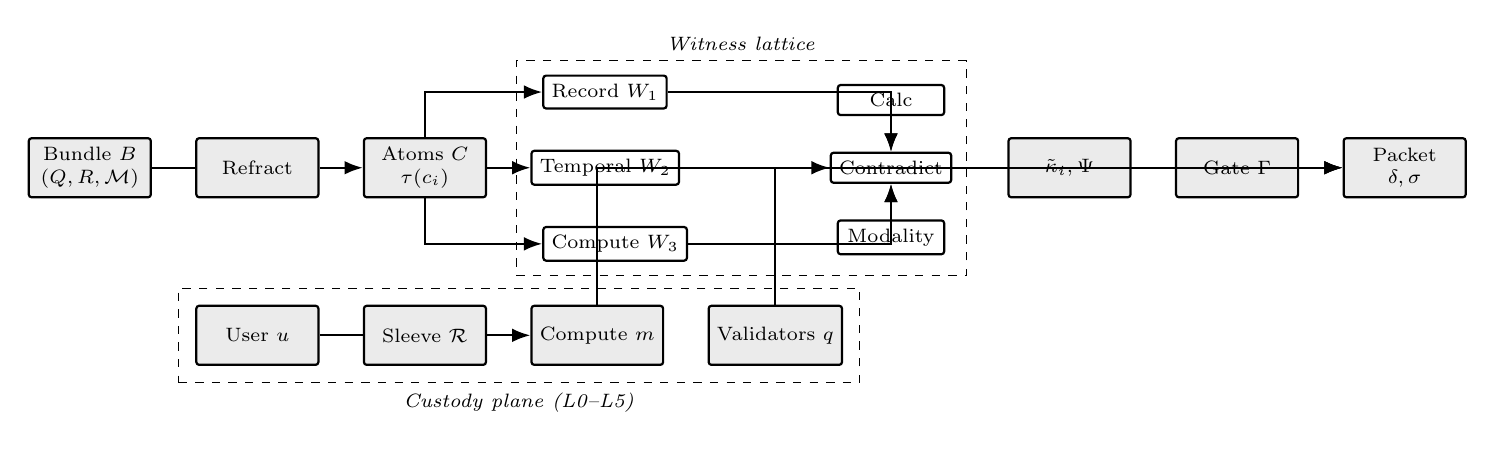
\begin{tikzpicture}[
  font=\scriptsize,
  box/.style={draw,thick,align=center,inner sep=3pt,rounded corners=1pt},
  hub/.style={box,fill=black!8,minimum width=1.55cm,minimum height=0.75cm},
  plane/.style={box,fill=white,minimum width=1.35cm},
  arr/.style={-{Latex},thick}
]
\node[hub] (b) {Bundle $B$\\$(Q,R,\mathcal{M})$};
\node[hub,right=0.55cm of b] (ref) {Refract};
\node[hub,right=0.55cm of ref] (c) {Atoms $C$\\$\tau(c_i)$};
\node[plane,above right=0.35cm and 0.7cm of c] (w1) {Record $W_1$};
\node[plane,right=0.55cm of c] (w2) {Temporal $W_2$};
\node[plane,below right=0.35cm and 0.7cm of c] (w3) {Compute $W_3$};
\node[plane,right=1.9cm of w2] (w4) {Contradict};
\node[plane,below=0.45cm of w4] (w5) {Modality};
\node[plane,above=0.45cm of w4] (calc) {Calc};
\node[hub,right=0.7cm of w4] (k) {$\tilde\kappa_i,\Psi$};
\node[hub,right=0.55cm of k] (g) {Gate $\Gamma$};
\node[hub,right=0.55cm of g] (p) {Packet\\$\delta,\sigma$};
\node[hub,below=1.35cm of c] (sl) {Sleeve $\mathcal{R}$};
\node[hub,left=0.55cm of sl] (u) {User $u$};
\node[hub,right=0.55cm of sl] (m) {Compute $m$};
\node[hub,right=0.55cm of m] (val) {Validators $q$};
\draw[arr] (b)--(ref)--(c);
\draw[arr] (c)|-(w1); \draw[arr] (c)--(w2); \draw[arr] (c)|-(w3);
\draw[arr] (w1)-|(w4); \draw[arr] (w2)--(w4); \draw[arr] (w3)-|(w4);
\draw[arr] (calc)--(w4); \draw[arr] (w5)--(w4);
\draw[arr] (w4)--(k)--(g)--(p);
\draw[arr] (u)--(sl)--(m); \draw[arr] (m)|-(p); \draw[arr] (val)|-(p);
\node[draw,dashed,fit=(u)(sl)(m)(val),inner sep=6pt,label=below:{\emph{Custody plane (L0--L5)}}] {};
\node[draw,dashed,fit=(w1)(w2)(w3)(w4)(w5)(calc),inner sep=5pt,label=above:{\emph{Witness lattice}}] {};
\end{tikzpicture}
\caption{Refraction Mesh: witness lattice (top) coupled to sleeve/custody plane and cosigned packet sealing (bottom).}
\label{fig:rma}
\end{figure*}

\subsection{Typed Atoms}
Each atom carries a type
\begin{equation}
\tau(c_i)\in\{\mathsf{text},\mathsf{vision},\mathsf{doc},\mathsf{table},\mathsf{calc},\mathsf{cross}\}.
\end{equation}
$\mathsf{calc}$ atoms are propositions about arithmetic or unit relations that should be checked by deterministic procedures, not only by another language model.
$\mathsf{cross}$ atoms assert consistency across modalities (e.g., ``the figure shows \$12M'' must match OCR/table and prose).

\subsection{Witness Planes}
A witness plane is a function
\begin{equation}
W_k:(c_i,\mathcal{S})\mapsto v_{i,k}\in\{\mathsf{support},\mathsf{contest},\mathsf{unknown}\},
\end{equation}
given source set $\mathcal{S}$.
RMA requires the following families for publication-bound work:
\begin{enumerate}
  \item Record plane (primary documents);
  \item Temporal plane (chronology / EXIF constraints);
  \item Compute plane (diverse weights or nodes);
  \item Contradiction plane (active disconfirmation)~\cite{schuster2021get};
  \item Modality plane (cross-modal consistency)~\cite{radford2021clip}.
\end{enumerate}

\subsection{Spectral Conflict Intensity}
Let
\begin{equation}
s_i=\lvert\{k:v_{i,k}=\mathsf{support}\}\rvert,\quad
t_i=\lvert\{k:v_{i,k}=\mathsf{contest}\}\rvert.
\end{equation}
Define spectral conflict intensity
\begin{equation}
\label{eq:kappa}
\kappa_i=\frac{t_i}{s_i+t_i+\varepsilon},\qquad \varepsilon>0.
\end{equation}
Under threshold $\tau_\kappa\in(0,1)$, claim $c_i$ is contested if $\kappa_i\ge\tau_\kappa$, or if any required plane returns $\mathsf{contest}$ when desk policy is strict.

\subsection{Packet Object}
A ProofPath packet is the tuple
\begin{equation}
\label{eq:packet}
P=\big(Q,R,\mathcal{M}_{\mathrm{handles}},C,\{(W_k,v_{i,k})\},\mathcal{N},G,\delta,\sigma\big),
\end{equation}
where $\mathcal{M}_{\mathrm{handles}}$ are content hashes (not necessarily raw bytes), $\mathcal{N}$ is the negative-evidence log, $G$ the gate decision, $\delta=\mathrm{MerkleRoot}(P\setminus\{\delta,\sigma\})$~\cite{merkle1987digital}, and $\sigma$ a set of Ed25519 cosignatures~\cite{edwards25519}.

\subsection{Orthogonality}
Let $E_k\in\{0,1\}$ be plane error indicators on a labeled contested set.
Empirical orthogonality is
\begin{equation}
\label{eq:omega}
\Omega = 1 - \frac{2}{m(m-1)}\sum_{1\le k<\ell\le m}\mathrm{Corr}(E_k,E_\ell).
\end{equation}
Low $\Omega$ diagnoses collapsed diversity (e.g., all compute planes calling one provider)~\cite{bender2021stochastic}.


\subsection{Weighted Spectral Measure and Soft Gate Score}
Not all planes are equal. Let $w_k>0$ be plane weights with $\sum_k w_k=1$. Define weighted support/contest mass
\begin{equation}
S_i=\sum_{k:v_{i,k}=\mathsf{support}} w_k,\qquad
T_i=\sum_{k:v_{i,k}=\mathsf{contest}} w_k,\qquad
U_i=\sum_{k:v_{i,k}=\mathsf{unknown}} w_k.
\end{equation}
The weighted conflict is
\begin{equation}
\label{eq:kappaW}
\kappa_i^{(w)}=\frac{T_i}{S_i+T_i+\varepsilon},\qquad
\tilde{\kappa}_i=\kappa_i^{(w)}\,(1-\alpha U_i),
\end{equation}
where $\alpha\in[0,1]$ down-weights conflict when ignorance dominates (unknown-heavy claims should tend to $\mathsf{review}$, not false $\mathsf{ready}$).

A soft publish score aggregates atoms:
\begin{equation}
\label{eq:soft}
\Psi(P)=\exp\!\Big(-\beta\sum_{i=1}^{n}\tilde{\kappa}_i\Big)\cdot\mathbf{1}\!\left[\min_i|\mathcal{W}_i|\ge q_{\min}\right],
\end{equation}
with temperature $\beta>0$. Hard gate $\Gamma$ can be recovered by thresholding $\Psi$ and applying the strict contest rule.

\subsection{Information Bound for Sleeve Unlinkability}
Let $U$ be requester identity, $M$ the multimodal payload, $L_m$ compute logs, and $R$ the relay transcript.
Under an honest-but-curious compute node and a correctly functioning sleeve,
\begin{equation}
\label{eq:mi}
I(U;L_m)\le I(U;R)+I(U;M\mid R).
\end{equation}
Private mode stores task hashes at the hub and strips transport identifiers at $\mathcal{R}$, driving the first term toward zero for local adversaries. The second term is controlled by minimization (handles): desks SHOULD ensure $M$ itself does not embed identifying metadata (EXIF GPS, named filenames).

\subsection{Consistency Functional Across Modalities}
For a cross-atom $c$ linking modalities $a,b$, define a consistency functional
\begin{equation}
\label{eq:cons}
\phi(c)=1-\frac{\|\,e_a(c)-e_b(c)\,\|_2}{\|e_a(c)\|_2+\|e_b(c)\|_2+\varepsilon},
\end{equation}
where $e_a,e_b$ are embeddings or normalized numeric feature maps (OCR totals, caption vectors, table aggregates).
Plane $W_{\mathrm{modality}}$ returns $\mathsf{contest}$ if $\phi(c)<\tau_\phi$.

\section{Multimodal Calculation Plane}
\label{sec:multi}

Multimodal desks do not only chat; they calculate.
Let $\mathrm{Calc}$ be a deterministic interpreter over extracted numeric relations:
\begin{equation}
\mathrm{Calc}(c_i)\mapsto\{\mathsf{match},\mathsf{mismatch},\mathsf{n/a}\}.
\end{equation}
We fold calc outcomes into spectral conflict by treating $\mathsf{mismatch}$ as a contesting vote.
This is a deliberate architectural choice: language models are strong at fluency and weak at reliable arithmetic consistency with tables~\cite{bender2021stochastic,openai2023gpt4}.
A calc veto is cheaper and more auditable than hoping a second model ``notices.''

\paragraph{Pipeline.}
(1)~content-address attachments;
(2)~run modality specialists (OCR, table parse, VQA) preferably on-node for restricted media;
(3)~refract into typed atoms;
(4)~schedule witness+calc planes;
(5)~log negative evidence;
(6)~apply $\Gamma$;
(7)~seal $(G,\delta,\sigma)$.
Streaming tokens remain a latency surface; sealed packets are the product of record.

\section{Decentralized Dual Fabric}
\label{sec:decentral}

\subsection{Principle}
\textbf{Decentralized-first, centralized-explicit.}
Self-hostable weights and independent nodes are the sovereignty path.
Centralized catalog routes may expand coverage but must never masquerade as local compute: both the UI and the packet label the route.

\subsection{Roles and Settlement}
Let roles be hub $\mathcal{H}$ (discovery, validator keys), relay $\mathcal{R}$ (sleeve hop), compute $\mathcal{C}$, witness feeds $\mathcal{F}$, and desk $\mathcal{D}$.
After inference, an attestation enters a Proof-of-Inference log.
Validators produce signatures; network-finality requires
\begin{equation}
\lvert\sigma\rvert \ge q,
\end{equation}
for configurable quorum $q$, in the spirit of Byzantine quora~\cite{castro1999pbft} but scoped to inference receipts rather than full SMR~\cite{nakamoto2008bitcoin}.

\subsection{Why Multimodality Raises the Stakes}
Images and sealed PDFs are high-value exfiltration targets.
Defaulting restricted multimodal inference to on-node routes reduces vendor retention surface area.
When a desk must use a centralized vision route, RMA requires: explicit labeling, packet provenance, optional sleeve, and never silent fallback.

\section{Data Protection Stack}
\label{sec:protect}

Product UIs often reduce ``privacy'' to a banner or a retention FAQ.
RMA instead treats custody as a layered protocol with explicit failure modes.
Let sensitivity class $\lambda(B)\in\{\mathsf{public},\mathsf{internal},\mathsf{restricted}\}$.

\subsection{Layer L0 --- Classification}
Before routing,
\begin{equation}
\rho(B)=
\begin{cases}
\mathsf{on\text{-}node}, & \lambda(B)=\mathsf{restricted},\\
\mathsf{prefer\text{-}node}, & \lambda(B)=\mathsf{internal},\\
\mathsf{any\text{-}labeled}, & \lambda(B)=\mathsf{public}.
\end{cases}
\end{equation}
Classification errors are themselves security bugs: over-labeling reduces utility; under-labeling violates G3.

\subsection{Layer L1 --- Privacy Sleeves (Data in Motion)}
Requester $u$ submits ciphertext task $\widetilde{T}$ to hub $\mathcal{H}$.
Relay $\mathcal{R}$ strips transport identity and forwards to compute $m\in\mathcal{C}$~\cite{chaum1981mix}.
Idealized unlinkability targets near-zero mutual information
\begin{equation}
I(U;\,L_m)\approx 0
\end{equation}
between requester identity $U$ and compute-side logs $L_m$ under private mode, acknowledging that global passive adversaries remain out of scope.

\subsection{Layer L2 --- Minimization and Handles}
Sealed packets store handles $h(m_j)=\mathrm{Hash}(m_j)$ and excerpts, not entire archives~\cite{benet2014ipfs}.
Raw blobs remain in desk-controlled storage with access control.
This separates \emph{auditability} from \emph{retention of pixels}.

\subsection{Layer L3 --- Encryption and Retention (Data at Rest)}
Desk artifacts (synced chats, exports) SHOULD be encrypted under desk keys.
Let retention clock $\mathcal{T}$ map artifact class to time-to-live.
Negative-evidence rows may outlive raw media when policy requires audit without keeping biometrics---a deliberate asymmetry.

\subsection{Layer L4 --- Route Provenance and UI Honesty}
Every reply and packet records route label
\begin{equation}
r\in\{\mathsf{decentralized}/\mathsf{on\text{-}node},\,\mathsf{centralized}/\mathsf{catalog}\}.
\end{equation}
Silent cross-cloud offload is a protocol violation even if the answer is ``correct.''
Honesty here is part of security, not marketing.

\subsection{Layer L5 --- Fail-Closed Private Desks}
Define availability predicate $A_{\mathrm{private}}$.
If $\lambda(B)=\mathsf{restricted}$ and $\neg A_{\mathrm{private}}$, then
\begin{equation}
\mathrm{Accept}(B)=\mathsf{false}.
\end{equation}
The system must refuse rather than ``helpfully'' send pixels to a public catalog.
Fail-open assistants optimize engagement; fail-closed desks optimize non-exfiltration.

\subsection{What This Stack Is Not}
Sleeves are not a substitute for endpoint security.
Screenshots bypass packet controls.
Differential privacy is not claimed for generative outputs~\cite{dwork2006differential}.
The contribution is a coherent custody control plane aligned with high-stakes desk practice.

\section{ProofPath Protocol}
\label{sec:proofpath}

ProofPath realizes RMA as an operational spiral:
\begin{enumerate}
  \item Atomize typed claims from $(R,\mathcal{M})$.
  \item Witness across required planes.
  \item Contradict with forced disconfirmation.
  \item Log negative evidence (empty searches are first-class)~\cite{silverman2015verification}.
  \item Persist extracts for third-party replay.
  \item Apply publish gate $\Gamma$.
\end{enumerate}

\begin{algorithm}[!t]
\caption{Multimodal ProofPath (simplified)}
\begin{algorithmic}[1]
\Require $Q,\mathcal{M},\Pi,\mathcal{S}$
\State classify $\lambda$; store handles $h(m_j)$
\If{$\lambda=\mathsf{restricted}$ \textbf{and} $\neg A_{\mathrm{private}}$}
\State \textbf{refuse} \Comment{L5 fail-closed}
\EndIf
\State $R\gets\mathrm{Infer}(Q,\mathcal{M})$ with labeled route $r$
\State $C\gets\mathrm{AtomizeTyped}(R,\mathcal{M})$
\ForAll{$c_i\in C$}
  \State collect $v_{i,k}\gets W_k(c_i,\mathcal{S})$ incl.\ calc/modality
  \State append contradiction + negative-evidence rows to $\mathcal{N}$
\EndFor
\State $G\gets\Gamma(P,\Pi)$; $\delta\gets\mathrm{MerkleRoot}(\cdot)$; solicit $\sigma$
\State \Return sealed $P$
\end{algorithmic}
\end{algorithm}

\section{Publish Gate Formalism}
\label{sec:gate}

Desk policy $\Pi=(\tau_\kappa,q_{\min},\mathcal{W}_{\mathrm{req}},\mathsf{strict})$ induces
\begin{equation}
\Gamma(P,\Pi)\in\{\mathsf{ready},\mathsf{review},\mathsf{blocked}\}.
\end{equation}
With $\mathcal{W}_i$ the set of planes that voted on $c_i$,
\begin{align}
\mathsf{blocked} &\Leftarrow \exists\,c_i:\ \kappa_i\ge\tau_\kappa\ \land\ \mathsf{strict},\\
\mathsf{ready} &\Leftarrow \forall\,c_i:\ \kappa_i<\tau_\kappa\ \land\ \lvert\mathcal{W}_i\rvert\ge q_{\min},\\
\mathsf{review} &\Leftarrow \text{otherwise}.
\end{align}
Export formats refuse $\mathsf{blocked}$ packets by default.
This encodes editorial caution as a predicate rather than as social hope~\cite{graves2017fact}.

\section{Security Analysis}
\label{sec:security}

\paragraph{Sybil witnesses.}
If anonymous web hits can cast gate-decisive votes, an adversary floods $\mathsf{support}$.
Therefore gate-decisive planes must be keyed to stake, institutional keys, or desk allowlists; raw web evidence remains advisory.

\paragraph{Model collusion.}
If all compute planes call one provider, orthogonality $\Omega$ collapses~\cite{bommasani2021foundation}.
Diversity labels and on-node options are mandatory for publish-critical work.

\paragraph{Poisoned multimodal evidence.}
Adversarial images and OCR spoofing are contested via modality and contradiction planes; calc mismatches fail closed under strict $\Pi$.

\paragraph{Privacy leakage.}
Sleeves reduce linkability~\cite{chaum1981mix}; extreme desks keep private routing fully on-prem~\cite{kairouz2021advances}.

\section{Novelty and Positioning}
\label{sec:novelty}

Scientific novelty in systems work is often compositional: a new arrangement of known primitives that enables new guarantees.
RMA's claim is of that kind---not a new backbone model, but a new control plane.
We state eight numbered positioning claims:

\begin{enumerate}
  \item[\textbf{N1}] \textbf{Typed multimodal atoms.}
  Unlike single-score chat and limited FEVER extractors~\cite{thorne2018fever,guo2022survey}, RMA refracts bundles into
  $\tau(c_i)\in\{\mathsf{text},\mathsf{vision},\mathsf{doc},\mathsf{table},\mathsf{calc},\mathsf{cross}\}$.

  \item[\textbf{N2}] \textbf{Deterministic calc veto.}
  Unlike RAG/LLM stacks that hope a second model notices arithmetic errors~\cite{lewis2020rag,openai2023gpt4},
  $\mathrm{Calc}$ can increment $t_i$ via $\mathsf{mismatch}$.

  \item[\textbf{N3}] \textbf{Orthogonal witness quora.}
  Unlike corpus-only checking~\cite{thorne2018fever}, publication requires multi-plane votes with measurable orthogonality $\Omega$ (Eq.~\eqref{eq:omega}).

  \item[\textbf{N4}] \textbf{Negative evidence as schema.}
  Unlike ephemeral UI traces, empty searches are first-class rows in $\mathcal{N}$~\cite{silverman2015verification}.

  \item[\textbf{N5}] \textbf{Export-blocking gate $\Gamma$.}
  Unlike soft scores, $\Gamma\in\{\mathsf{ready},\mathsf{review},\mathsf{blocked}\}$ can refuse export under $\kappa_i\ge\tau_\kappa$~\cite{graves2017fact}.

  \item[\textbf{N6}] \textbf{Durable cosigned packets.}
  Unlike multi-agent debate that discards intermediate turns~\cite{wei2022chain,chen2023agents}, RMA seals $(G,\delta,\sigma)$ for replay.

  \item[\textbf{N7}] \textbf{Structured epistemic notarization.}
  Unlike ledger blob timestamps alone~\cite{nakamoto2008bitcoin,buterin2014ethereum}, cosigning covers claims, votes, absences, and gate---not only existence at time $t$.

  \item[\textbf{N8}] \textbf{Fail-closed custody protocol.}
  Unlike ``private chat'' product modes, layers L0--L5 encode classification, sleeves~\cite{chaum1981mix}, handles, encryption, route honesty, and $\mathrm{Accept}(B)=\mathsf{false}$ when private capacity is missing.
\end{enumerate}

\begin{table*}[!t]
\centering
\caption{Tractable measures of verification and custody (physical/operational units).
Bit = indicator in $\{0,1\}$. Unbounded MI = no sleeve architecture. RMA entries are invariants or evaluation targets.}
\label{tab:compare}
\renewcommand{\arraystretch}{1.12}
\setlength{\tabcolsep}{3.5pt}
\begin{tabular}{@{}p{4.6cm}ccc@{}}
\toprule
Measure (unit) & LLM chat & FEVER/RAG & RMA \\
\midrule
Witness planes for publish $m$ (count) & $0$ & $1$ & $\ge 2$ \\
Typed atom families $|\mathcal{T}|$ (count) & $1$ & $1$ & $6$ \\
Calc$\to$contest coupling (bit) & $0$ & $0$ & $1$ \\
Neg.-evidence rows $|\mathcal{N}|$ if searched (count) & $0$ & $0$ & $\ge 1$ \\
Export block if $\kappa_i\ge\tau_\kappa$ (bit) & $0$ & $0$ & $1$ \\
Merkle digest $|\delta|$ (bits) & $0$ & $0$ & $256$ \\
Cosign quorum $q$ (signatures) & $0$ & $0$ & $\ge 1$ \\
Route label on reply (bit) & $0$ & $0$ & $1$ \\
Refuse if $\neg A_{\mathrm{private}}$ (bit) & $0$ & $0$ & $1$ \\
Sleeve $I(U;L_m)$ (nats, private) & unbdd. & unbdd. & $\to 0$ \\
Orthogonality $\Omega$ (dimensionless) & n/a & $\sim 0$ & $\uparrow 1$ \\
Replay fidelity of $\delta$ (\%) & n/a & n/a & $\ge 99$ \\
Warm ProofPath $T_{90}$ (s) & n/a & n/a & $\le 90$ \\
False-ready @ strict $\Pi$ (\%) & n/a & n/a & $<5$ \\
\bottomrule
\end{tabular}
\end{table*}

\section{Worked Example}
\label{sec:example}

Consider prose asserting that ``Mayor Reyes diverted \$12M of transit funds to a private foundation in March 2025,'' accompanied by a budget PDF page image.
Refraction yields $c_1$ (amount), $c_2$ (date), $c_3$ (destination), $c_4$ (attribution), and a $\mathsf{cross}/\mathsf{calc}$ atom linking OCR totals to prose.
If the temporal plane contests March while calc matches \$12M, then $\kappa_2$ rises.
Under strict $\Pi$, $\Gamma$ returns $\mathsf{blocked}$ until the date is resolved.
An empty FOIA index query enters $\mathcal{N}$---absence as evidence~\cite{silverman2015verification}.

\section{Implementation and Evaluation Agenda}
\label{sec:impl}

The Noeti deployment maps RMA onto a discovery hub, Chat and spatial Canvas surfaces, ProofPath Desk, on-node open weights, a labeled network catalog, and live wire feeds.
Proposed metrics include gate precision/recall on journalist-labeled contested claims~\cite{thorne2018fever}; replay fidelity of $\delta$; orthogonality $\Omega$; sleeve efficacy $I(U;L_m)$; calc-plane catch rate; and restricted-mode refusal rate when only centralized vision routes exist.

\section{Limitations and Ethics}
\label{sec:ethics}

RMA structures disagreement; it does not mint truth~\cite{graves2017fact}.
Over-confident gates can suppress legitimate contested reporting; under-confident gates fail the beachhead.
Human editors retain authority~\cite{silverman2015verification}.
If pixels leave the desk, the packet must say so---otherwise privacy UI becomes security theatre.

\section{Conclusion}
\label{sec:concl}

We presented the Refraction Mesh Architecture as a research systems design for multimodal, decentralized, custody-aware claim verification.
By refracting composites into typed atoms, measuring spectral conflict across orthogonal planes, protecting data through a fail-closed stack, and sealing publish decisions under Proof-of-Inference cosignatures, RMA offers high-stakes desks a path to use generative models without surrendering either epistemic standards or case files to a single cloud.

\section*{Acknowledgment}
Correspondence: \texttt{dev@noeticompute.com}. Implementation surface: \url{https://noeticompute.com}.

\bibliographystyle{IEEEtran}
\bibliography{refs}

\end{document}
